\documentclass{article}[12pt]
\usepackage{color}
\usepackage[normalem]{ulem}
\usepackage{times}
\usepackage{fullpage}
\usepackage{listings}
\usepackage{amsmath}
\usepackage{amssymb}
\usepackage{tikz}
\def \R {\mathbb R}
\def \imp {\Longrightarrow}
\def \eps {\varepsilon}
\def \Inf {{\sf Inf}}
\newenvironment{proof}{{\bf Proof.  }}{\hfill$\Box$}
\newtheorem{theorem}{Theorem}[section]
\newtheorem{definition}{Definition}[section]
\newtheorem{corollary}{Corollary}[section]
\newtheorem{lemma}{Lemma}[section]
\newtheorem{claim}{Claim}[section]
\setlength {\parskip}{2pt}
\setlength{\parindent}{0pt}

\newcommand{\headings}[4]{\noindent {\bf Assignment 12 CME241} \hfill {{\bf Author:} Nicolas Sanchez} \\
{} \hfill {{\bf Due Date:} #2} \\

\rule[0.1in]{\textwidth}{0.025in}
}

\newcommand{\klnote}[1]{{\color{red} #1}}
\newcommand{\klsout}[1]{{\color{red} \sout{#1}}}

\begin{document}

\headings{\#1}{Tuesday, October 8, 10:30am}\section{} 



\section{n-step and TD($\lambda$) implementation}
We implement the n-step and TD lambda (tabular case) in the algorithms as suggested:

\begin{lstlisting}
def n_step_prediction(
        traces: Iterable[Iterable[mp.TransitionStep[S]]],
        n_steps: int,
        approx_0: FunctionApprox[S],
        gamma: float,
        tolerance: float,
) -> Iterator[FunctionApprox[S]]:
        func_approx: FunctionApprox[S] = approx_0
    max_steps  = round(math.log(tolerance) / math.log(gamma)) if gamma < 1 else 10000

    for trace in traces:
        # these will be sliding windows to look at n-long windows
        relevant_states = []
        relevant_rewards = []
        
        #these will be fed into function approximation
        predictors: List[S] = []
        responses: Sequence[float] = []

        t = 0
        for tr in trace:
            if t > max_steps:
                break
            if t < n_steps:
                # gather enough step for n-step bootstrapping
                relevant_states.append(tr.state)
                relevant_rewards.append(tr.reward)
            else:

                # record the pair
                predictors.append(relevant_states[0])
                rew = (gamma**n_steps)*func_approx(tr.state)
                for i in range(n_steps):
                    rew += (gamma**i)*relevant_rewards[i]
                responses.append(rew)

                # update the sliding window
                relevant_states.append(tr.state)
                relevant_rewards.append(tr.reward)
                relevant_states = relevant_states[1:]
                relevant_rewards = relevant_rewards[1:]
            t+=1

        func_approx = func_approx.update(zip(predictors, responses))
        yield func_approx
        
def td_lambda_prediction_tabular(
        traces: Iterable[Iterable[mp.TransitionStep[S]]],
        approx_0: FunctionApprox[S],
        gamma: float,
        lambd: float,
        tolerance:float,
        learning_rate: Callable[[int], float],
        max_traces: int
) -> Iterator[FunctionApprox[S]]:

    values_dict = {}
    max_steps  = round(math.log(tolerance) / math.log(gamma)) if gamma < 1 else 10000
    step_num = 0
    trace_num = 0
    for trace in traces:
        trace_eligibility : Dict[S,float] = {}
        if trace_num > max_traces:
        	break
        #these will be fed into function approximation
        if step_num % 100 == 0:
            print(step_num)
            print(values_dict)
            print(max_steps)
        t = 0
        for tr in trace:
            if t > max_steps:
                break
            td_error = tr.reward + gamma*values_dict.get(tr.next_state,0) - values_dict.get(tr.state,0)
            
            if tr.state not in trace_eligibility:
                trace_eligibility[tr.state] = 0.
            for state in trace_eligibility:
                if state == tr.state:
                    trace_eligibility[tr.state] = gamma*lambd*trace_eligibility[state] + 1.
                else:
                    trace_eligibility[state] = gamma*lambd*trace_eligibility[state]
                # print(learning_rate(step_num)*td_error*trace_eligibility[state])
                values_dict[state] = values_dict.get(state,0.) + learning_rate(step_num)*td_error*trace_eligibility[state]
            step_num+=1
            t+=1
        trace_num += 1
    return values_dict
\end{lstlisting}

We test our implementation with the inventory problem and recover similar values confirm first level of correctness:

\begin{figure}[h]
  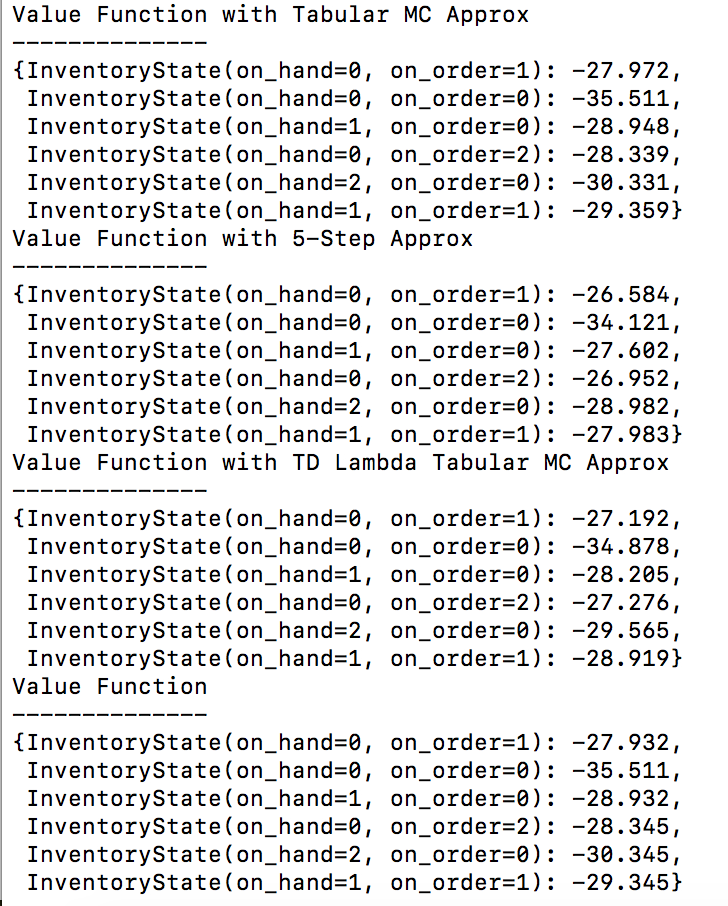
\includegraphics[width=0.5\linewidth]{correctness.png}
  \caption{Convergence of three control methods}
  \label{fig:optPol1}
\end{figure}

\section{MC Error and discounted TD errors derivation}
We derive:

\begin{align*}
G_t - V(S_t)  & = \sum_{u=t}^{T-1}\gamma^{u-t}R_{u+1} - V(S_t) & \text{ by definiton of $G_t$}\\
& = \sum_{u=t}^{T-1}\gamma^{u-t}R_{u+1} - V(S_t) + \sum_{u = t+1}^{T}\gamma^{u-t}(V(S_u) - V(S_{u}))& \text{ since we are adding 0}\\
& = \sum_{u=t}^{T-1}\gamma^{u-t}R_{u+1} - V(S_t) + \sum_{w = t+1}^{T}\gamma^{w-t}V(S_w) - \sum_{k = t+1}^{T}\gamma^{k-t}V(S_k) & \text{ by distributive property}\\
& = \sum_{u=t}^{T-1}\gamma^{u-t}R_{u+1} - \sum_{w = t}^{T}\gamma^{w-t}V(S_w) + \sum_{k = t+1}^{T}\gamma^{k-t}V(S_k) & \text{ by incorporating the first term}\\
& = \sum_{u=t}^{T-1}\gamma^{u-t}R_{u+1} - \sum_{w = t}^{T-1}\gamma^{w-t}V(S_w) + \sum_{k = t+1}^{T}\gamma^{k-t}V(S_k) & \text{ since $V(S_T) = 0$ for terminal state}\\
& = \sum_{u=t}^{T-1}\gamma^{u-t}R_{u+1} + \sum_{w = t}^{T-1}(-\gamma^{w-t}V(S_w) + \gamma^{w+1-t}V(S_{w+1})) & \text{ by combining sums}\\
& = \sum_{w=t}^{T-1}\gamma^{u-t}R_{u+1} + (-\gamma^{u-t}V(S_u) + \gamma^{u+1-t}V(S_{u+1})) & \text{ by combining sums}\\
& = \sum_{u=t}^{T-1}\gamma^{u-t}(R_{u+1} + \gamma V(S_{u+1}) -V(S_u) ) & \text{ by factoring out}\\
\end{align*}
Which is the desired equality.



\end{document}
